\documentclass[11pt]{article}
\usepackage[utf8]{inputenc}\usepackage[T1]{fontenc}
\usepackage{amsmath,amssymb,amsthm}\usepackage[margin=1in]{geometry}
\usepackage{graphicx}\usepackage{booktabs}
\usepackage[hidelinks]{hyperref}
\newtheorem{theorem}{Theorem}\newtheorem{definition}{Definition}

\title{The Factor Statistics of Twin Centres on the $6N$ Skeleton:\\
Each Prime Divides with Probability $1/(q-2)$, not $1/q$}
\author{Ruqing Chen\\
\small GUT Geoservice Inc., Montreal, Quebec, Canada\\
\small \texttt{ruqing@hotmail.com}}
\date{\today}

\begin{document}
\maketitle

\begin{abstract}
Throughout Parts~I--XI the factor count $\omega_{>3}(N)$ was used as a given
stratum. Here we ask what distribution it follows for the sparse set of twin
centres themselves. The answer is a single clean replacement: a prime $q>3$
divides a twin centre with probability $1/(q-2)$, against $1/q$ for an ordinary
integer. We verify this per prime on the $2.4\times10^{7}$ twin centres of
$S_{10}$ (and $S_9$): for small $q$ the measured $P(q\mid N,\,N\text{ twin})$
equals $1/(q-2)$ to within $0.1\%$. This is the microscopic root of the Part~I
enrichment factor $\prod(q-1)/(q-3)$, which is exactly the product of these raised
single-prime probabilities. The consequent rightward shift of the mean has the
convergent closed form $\sum_{q>3}\bigl(\tfrac1{q-2}-\tfrac1q\bigr)=0.2604$; the
finite-$N$ measured shift increases with the shell ($+0.222$ on $S_9$, $+0.227$ on
$S_{10}$), approaching the closed form as the large-$q$ truncation recedes. We do
\emph{not} claim a normal law: at the accessible scale $\ln\ln(6N)\approx3$ the
distribution has not reached its Erd\H{o}s--Kac limit (mean $\ne$ variance,
nonzero skew), and the limiting law is left open. No claim is made about the
infinitude of twin primes.
\end{abstract}

\section{The single-prime probability}

For an ordinary integer, a prime $q$ divides it with probability $1/q$. A twin
centre $N$ is constrained: $6N\mp1$ must both be prime, so modulo $q>3$ the
residue of $N$ must avoid the two forbidden classes
$\mathrm{dead}(q)=\{\pm6^{-1}\bmod q\}$, leaving $q-2$ admissible residues. The
residue $0$ (i.e.\ $q\mid N$) is one of these admissible classes, and within them
no class is locally favoured for twin-ness at $q$. Hence:

\begin{theorem}[single-prime divisibility]\label{thm:prob}
For $q>3$, $\ \displaystyle P(q\mid N \mid N\text{ twin})=\frac{1}{q-2}.$
\end{theorem}

Measured on $S_{10}$ ($23{,}988{,}173$ twin centres) and $S_9$, the equality holds
per prime to high precision (Table~\ref{tab:perq}, Fig.~\ref{fig:omega} left): for
$q\le 401$ the ratio of the measured probability to $1/(q-2)$ is within $0.4\%$
($0.1\%$ for the smallest, most frequent $q$), tightening from $S_9$ to $S_{10}$.
For large $q$ the per-prime measurement is dominated by sampling depletion
($P\sim1/q$ gives only tens of divisible centres at $q\sim10^5$), and is not a
deviation from the law.

\begin{table}[h]\centering\small
\begin{tabular}{rcccc}
\toprule
$q$ & $1/q$ (ord.) & $1/(q-2)$ & meas $S_{10}$ & ratio\\
\midrule
5  & 0.20000 & 0.33333 & 0.333349 & 1.0000\\
7  & 0.14286 & 0.20000 & 0.200004 & 1.0000\\
11 & 0.09091 & 0.11111 & 0.111090 & 0.9998\\
13 & 0.07692 & 0.09091 & 0.090895 & 0.9998\\
17 & 0.05882 & 0.06667 & 0.066597 & 0.9990\\
19 & 0.05263 & 0.05882 & 0.058812 & 0.9998\\
23 & 0.04348 & 0.04762 & 0.047595 & 0.9995\\
47 & 0.02128 & 0.02222 & 0.022217 & 0.9998\\
97 & 0.01031 & 0.01053 & 0.010521 & 0.9994\\
401 & 0.00249 & 0.00251 & 0.002517 & 1.0044\\
\bottomrule
\end{tabular}
\caption{$P(q\mid N\mid N\text{ twin})$ on $S_{10}$ equals $1/(q-2)$, not the
ordinary $1/q$. Small $q$ confirm the law to $\le0.4\%$; large $q$ (not shown
past $401$) are sampling-limited.}
\label{tab:perq}
\end{table}

\section{Root of the Part~I enrichment}

Theorem~\ref{thm:prob} is the microscopic source of the macroscopic enrichment of
Part~I. The relative density of twin centres among integers divisible by $q$ over
those not is, from the raised probability,
\[
  \frac{P(q\mid N\mid\text{twin})}{P(q\nmid N\mid\text{twin})}\Big/
  \frac{1/q}{1-1/q}
  =\frac{q-1}{q-3},
\]
so the conditional density carries the factor $\prod_{q\mid N}(q-1)/(q-3)$ first
measured in Part~I. The enrichment is precisely the product of the single-prime
probability boosts $1/q\to1/(q-2)$.

\section{The mean shift}

Since $\omega_{>3}(N)=\sum_{q>3}\mathbf 1\{q\mid N\}$, the mean shift between twin
centres and ordinary integers is, term by term,
\[
  \langle\omega_{>3}\rangle_{\text{twin}}-\langle\omega_{>3}\rangle_{\text{ord}}
  =\sum_{q>3}\Bigl(\frac1{q-2}-\frac1q\Bigr)=0.2604,
\]
a convergent constant (each term $\sim 2/q^2$), independent of any cutoff---unlike
the individual means, which diverge as $\ln\ln$. The measured finite-$N$ shift is
smaller and grows with the shell: $+0.2220$ on $S_9$, $+0.2270$ on $S_{10}$
(Table~\ref{tab:sum}). The deficit from $0.2604$ is the contribution of large
primes $q$ whose divisibility is truncated by the finite range $N\le H$; as $H$
grows these terms are recovered, and the two-shell trend confirms the approach to
the closed form.

\begin{table}[h]\centering\small
\begin{tabular}{lcccccc}
\toprule
shell & ord.\ mean & twin mean & shift & twin var & twin skew & twin ex.kurt\\
\midrule
$S_9$    & 2.3599 & 2.5819 & $+0.2220$ & 0.9423 & $0.246$ & $-0.326$\\
$S_{10}$ & 2.4757 & 2.7027 & $+0.2270$ & 1.0394 & $0.258$ & $-0.287$\\
\bottomrule
\end{tabular}
\caption{Mean shift grows toward the closed form $0.2604$ with shell depth. The
normality diagnostics (mean $\ne$ var, nonzero skew/kurtosis) show the
Erd\H{o}s--Kac limit is not reached at this scale.}
\label{tab:sum}
\end{table}

\begin{figure}[h]\centering
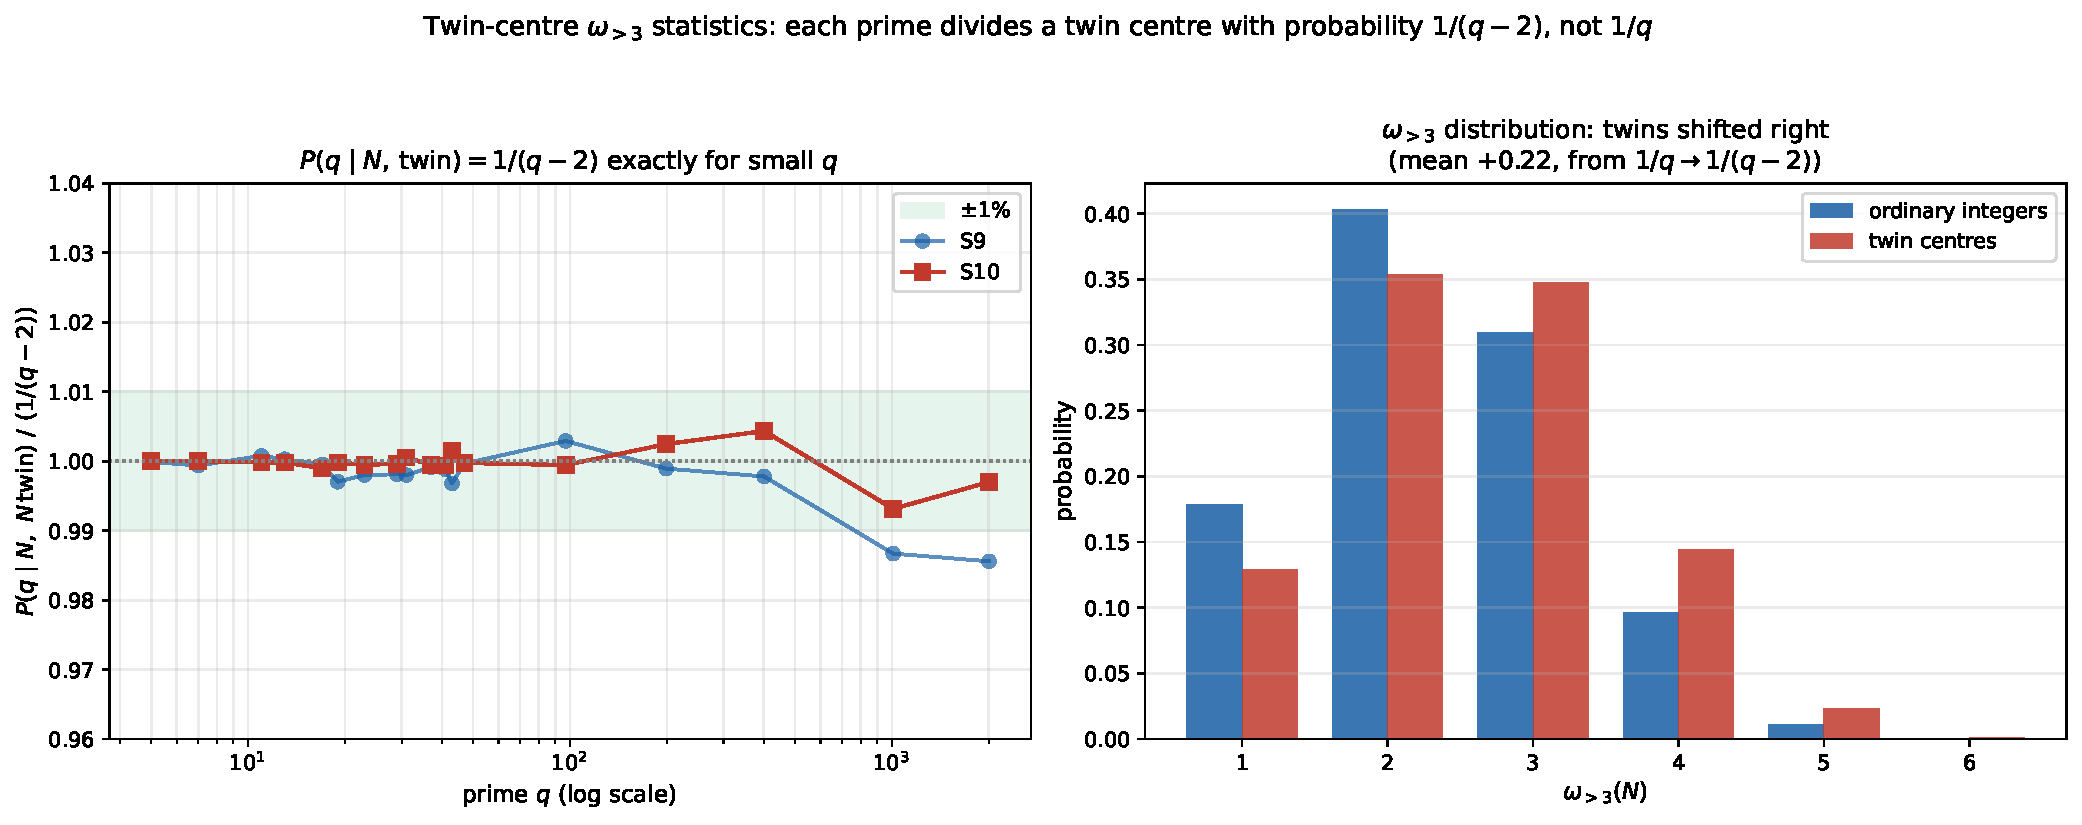
\includegraphics[width=\textwidth]{fig_paper12_omega.pdf}
\caption{Left: $P(q\mid N,\text{twin})/(1/(q-2))$ versus $q$, both shells; flat at
$1$ for small $q$, sampling-limited at large $q$. Right: the $\omega_{>3}$
distribution of twin centres (red) is shifted right of ordinary integers (blue).}
\label{fig:omega}
\end{figure}

\section{Normality is not claimed}

One might expect $\omega_{>3}$ of twin centres to follow an Erd\H{o}s--Kac normal
law with Bernoulli parameter $1/(q-2)$. We do \emph{not} assert this. At the
accessible scale the mean ($2.70$) and variance ($1.04$) are far apart, and the
skewness ($+0.26$) and excess kurtosis ($-0.29$) are nonzero; with
$\ln\ln(6N)\approx3$ the distribution is far from its limit, for ordinary integers
as much as for twins. The limiting law of $\omega_{>3}$ over twin centres---and
whether the natural variance $\sum 1/(q-2)\bigl(1-1/(q-2)\bigr)$, constrained by
the finite number of prime factors, governs it---is left as an open problem.

\section{Conclusion}

Twin centres carry a clean factor statistic: each prime $q>3$ divides one with
probability $1/(q-2)$ rather than $1/q$, verified per prime on $S_9$ and $S_{10}$
to within $0.4\%$ for the dominant small primes. This is the microscopic origin of
the Part~I enrichment $\prod(q-1)/(q-3)$, and it shifts the mean $\omega_{>3}$
rightward by the convergent constant $\sum_{q>3}(1/(q-2)-1/q)=0.2604$, approached
from below as the shell deepens. We make no normality claim: at this scale the
Erd\H{o}s--Kac limit is not reached, and the limiting distribution is open. As
throughout this series, no claim is made about the infinitude of twin primes or
any $k$-tuple conjecture; this is a measured, factor-resolved account of the
arithmetic of the twin skeleton.

\paragraph{Data and code availability.}
The per-prime probabilities and the $\omega$ distribution are openly
available~\cite{repo}; the $S_{10}$ twin count $23{,}988{,}173$ matches Part~I.

\begin{thebibliography}{9}
\bibitem{ChenI} R.~Chen, \emph{Prime distribution on the $6N$ skeleton} (Part~I),
Zenodo, doi:10.5281/zenodo.20470367 (2026).
\bibitem{ChenVIII} R.~Chen, \emph{The arithmetic structure of the bridge
constant} (Part~VIII), Zenodo, doi:10.5281/zenodo.20519998 (2026).
\bibitem{ChenXI} R.~Chen, \emph{The first-principles origin of the tail constant}
(Part~XI), Zenodo, doi:10.5281/zenodo.20526835 (2026).
\bibitem{EK} P.~Erd\H{o}s, M.~Kac, \emph{The Gaussian law of errors in the theory
of additive number theoretic functions}, Amer.\ J.\ Math.\ \textbf{62} (1940),
738--742.
\bibitem{repo} R.~Chen, \emph{$6N$ twin-centre factor statistics: data and code},
\url{https://github.com/Ruqing1963/6N-twin-centre-omega}  (2026).
\end{thebibliography}

\end{document}
